\chapter{Asking Wall Street Millionaires How To Make \$1 Million}

This episode is not a blackboard lecture, but it does possess a real internal mathematics. The speaker applies the same operator to a sequence of people on Wall Street: when did you make your first million, by what mechanism did it happen, and what would you tell somebody trying to do the same now? Out of that repeated questioning there gradually emerges a compact theory of commercial life: persistence under refusal, centralization and scale in a service business, the distinction between a windfall and a durable flow, the economics of professional practice, the leverage of distribution, and finally the private-equity insistence on actual cash generation rather than decorative earnings.

\section{Opening Question and Search Friction}

The lecture first gives us outcomes before mechanisms. We hear of finance, private equity, a television network in airports and hotels, and a year in which \$250 million was made. We hear also a different kind of claim: somebody who made a first million only about a decade ago, sold everything, and started again. The teaser therefore does not answer the main question; it tells us only that the sample space is broad.

Once the speaker stands on Wall Street and states the day's plan, the method becomes clear. We shall ask the same question repeatedly and let the answers separate themselves. What stays fixed is the probe: age at the first million, line of business, and advice for making one now. What varies is access. Some people refuse, some evade, some joke, some give partial signal and disappear. This is not wasted footage. It establishes the first principle of the lecture: useful commercial information is scarce not because it does not exist, but because it is embedded in moving people, guarded by time pressure, and available only to a sufficiently persistent search.

In that sense the lecture begins not with wealth but with search cost. Before we can extract a business mechanism, we must first survive refusal.

\section{From ``No'' to ``Not Yet''}

After the first round of failed approaches, the speaker does something structurally important: he pauses the street hunt and interprets it. Yesterday did not go as planned, he says, but the operative lesson is not defeat. The lecture's first genuine update rule is psychological and procedural at once:
\begin{equation}
\text{No}_t \longmapsto \text{Not Yet}_{t+1}.
\end{equation}
A refusal is no longer treated as a terminal theorem; it is treated as a change of state.

\begin{figure}[h]
\centering
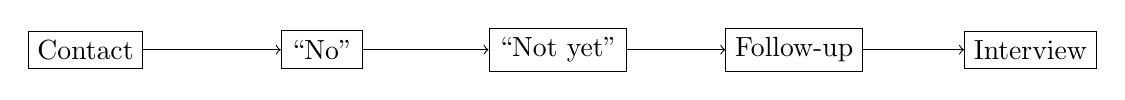
\begin{tikzpicture}
\node[draw, rectangle] (c) at (0,0) {Contact};
\node[draw, rectangle] (n) at (3,0) {``No''};
\node[draw, rectangle] (ny) at (6,0) {``Not yet''};
\node[draw, rectangle] (f) at (9,0) {Follow-up};
\node[draw, rectangle] (i) at (12,0) {Interview};
\draw[->] (c) -- (n);
\draw[->] (n) -- (ny);
\draw[->] (ny) -- (f);
\draw[->] (f) -- (i);
\end{tikzpicture}
\end{figure}

The point of this figure is modest but exact. If the search process terminates at the first refusal, no mechanism is ever observed. If refusal is recoded as delay, the process remains alive long enough for a real case to appear. That is why the lecture moves from a recap of failure directly into day two on Wall Street. The persistence is not ornamental motivation; it is the condition under which the later business models become visible.

\section{Dry Cleaning as a Scalable System}

The first substantial case is not a hedge fund or a glamorous software startup. It is dry cleaning. This is important. The lecture wants its first real mechanism to come from an ordinary service business, because that makes the logic of scale easier to see. The guest says he once had ten dry cleaners, and when the speaker asks how one gets from one site to ten, the answer is immediate and concrete: own the factory.

\subsection{Question \& Answer}

\paragraph{Question.} How do we scale a small service business without duplicating the expensive core ten times?

\paragraph{Answer.} We separate the edge of the business from the center of the business. The storefront is not the true production site. It is a collection point, a tagging-and-bagging point, a retail interface. The factory is where the real work is done. Once that separation is made, scale ceases to mean ``build ten full businesses'' and begins to mean ``build one production core and many intake nodes.''

\begin{figure}[h]
\centering
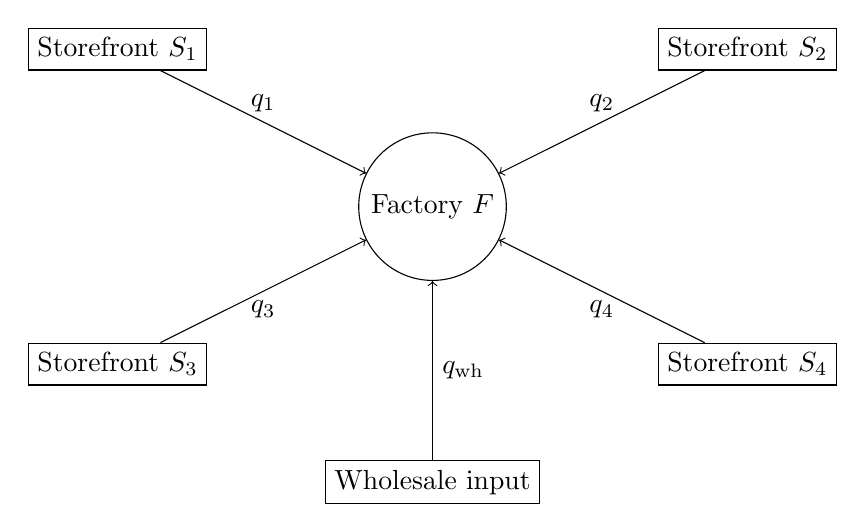
\begin{tikzpicture}
\node[draw, circle] (f) at (0,0) {Factory $F$};
\node[draw, rectangle] (s1) at (-4,2) {Storefront $S_1$};
\node[draw, rectangle] (s2) at (4,2) {Storefront $S_2$};
\node[draw, rectangle] (s3) at (-4,-2) {Storefront $S_3$};
\node[draw, rectangle] (s4) at (4,-2) {Storefront $S_4$};
\node[draw, rectangle] (w) at (0,-3.5) {Wholesale input};
\draw[->] (s1) -- node[above] {$q_1$} (f);
\draw[->] (s2) -- node[above] {$q_2$} (f);
\draw[->] (s3) -- node[below] {$q_3$} (f);
\draw[->] (s4) -- node[below] {$q_4$} (f);
\draw[->] (w) -- node[right] {$q_{\mathrm{wh}}$} (f);
\end{tikzpicture}
\end{figure}

We can write the stripped-down throughput model as
\begin{align}
Q &= \sum_{i=1}^{n} q_i, \qquad n_{\text{cleaners}} = 10, \\
R_{\text{network}} &= p_{\text{shirt}}\,Q, \qquad p_{\text{shirt}} \approx 1.99\ \text{USD}, \\
\Pi_{\text{network}} &= p_{\text{shirt}}Q - c_{\text{unit}}Q - C_F - \sum_{i=1}^{n} C_{S_i} - C_{\text{transport}}.
\end{align}
Here $F$ is the factory, $S_i$ is storefront $i$, $q_i$ is the monthly intake at that storefront, and $Q$ is the system-wide throughput. The lecture gives a rough unit-cost figure of about $0.40$ dollars, though the transcript is verbally rough at precisely that point.

\begin{remark}
The arithmetic here is illustrative rather than definitive. The lecture does not provide a full cost stack, labor schedule, rent schedule, or mix of services. We are preserving the mechanism, not pretending to have recovered a complete profit-and-loss statement.
\end{remark}

Still, the guest makes a quantitative claim sharp enough to test. He says that with this structure one can run a $500$ square foot place and still make about $50{,}000$ dollars a month. If we momentarily suppress fixed costs and simply compute the contribution margin, we obtain
\begin{align}
m &= p_{\text{shirt}} - c_{\text{unit}} \approx 1.99 - 0.40 = 1.59\ \text{USD}, \\
Q^\star &\approx \frac{50{,}000}{1.59} \approx 3.14\times 10^4\ \text{garments/month}, \\
\frac{Q^\star}{30} &\approx 1.05\times 10^3\ \text{garments/day}.
\end{align}
This is not a proof that the business produces exactly that monthly profit. It is better understood as a consistency check. The lecture's number presumes serious throughput, and very likely a broader service mix or wholesale flow, but it also shows why the structure matters. Once the factory is centralized, each storefront is a volume collector rather than a miniature plant.

The guest then adds a second scaling insight. If the factory is good enough, even apparent competitors can become wholesale customers. The lecture thereby widens the model: a competitor need not remain outside the system. It can be pulled into the throughput term $Q$.

\section{From First Million to Durable Flow}

The dry-cleaning interview does not stop at the first million. The speaker pushes past the making of money to the keeping of money, and the guest answers by resisting the usual frame. When asked what to invest in, he does not begin with portfolios, asset classes, or leverage. He begins with behavior: do not chase reaction, do not imagine that one quick win is a stable life, do not let money turn into theater.

\subsection{Question \& Answer}

\paragraph{Question.} If one can make a great deal of money in a single year, what makes that wealth repeatable rather than temporary?

\paragraph{Answer.} The lecture's answer is almost anti-financial at first glance. It treats preservation not as an optimization over returns but as a constraint on identity drift and spending drift. A simple bookkeeping form is enough:
\begin{equation}
W_{t+1} = W_t + CF_t - C_t.
\end{equation}
Here $W_t$ is wealth, $CF_t$ is the cash generated by the operating system, and $C_t$ is consumption.

The guest's practical claim is that new money often enlarges $C_t$ without strengthening the business process that produced $CF_t$. A one-time event can therefore masquerade as a durable equilibrium. The safe condition is elementary:
\begin{equation}
\Delta W_t > 0 \qquad \Longleftrightarrow \qquad CF_t > C_t.
\end{equation}
But the lecture wants us to notice something subtler. The dangerous variable is often not business weakness but performative consumption. Hence the deliberately ordinary examples: driving a Kia in New York rather than buying a Lamborghini for cobblestone streets, still eating the same neighborhood pizza after wealth arrives, refusing to spend in order to look newly rich.

That is why the speaker's question ``What do you invest in?'' is met with a partial rejection. The guest's answer is that preservation begins earlier than an investment decision. It begins with remaining continuous with oneself. In the language of the lecture, do not become weird. This is rough street language, but the mechanism is precise: if the operating system continues to produce cash while the expenditure baseline remains disciplined, the flow survives.

\section{Professional Practice, Purpose, and the Long Horizon}

The next major case is different in kind. A spine surgeon says he made many millions only in the last year, then explains the business lesson he would give to somebody emerging from medical school with what the speaker calls shiny-object syndrome. The reply is forward-looking and anti-consumerist: plan for the future, since today's sunshine may become tomorrow's rain; do not chase objects; happiness lies in the pursuit of purpose.

Two further mechanisms appear here. The first is entrepreneurial: the jump in income came when he started his own practice. The second is commercial: he does not describe himself as selling. His line is that the product sells itself because he takes care of people. We can write the logic schematically as
\begin{align}
\text{care quality} &\longrightarrow \text{trust}, \\
\text{trust} &\longrightarrow \text{patients and referrals}, \\
\text{patients and referrals} &\longrightarrow CF_{\text{actual}}.
\end{align}
This is not a law of medicine alone. It is the lecture's more general proposition that sustained demand can emerge from service quality rather than aggressive closing.

The surgeon is also the clearest speaker on the relation between preservation and self-comparison. When asked how he preserves wealth, he answers: by being better than he was yesterday. We can record the form of that idea schematically as
\begin{equation}
\Delta_{\text{self}}(t) = \text{performance}(t) - \text{performance}(t-1).
\end{equation}
The lecture does not turn this into a formal optimization problem, but the benchmark is clear. The relevant comparison is not with the rival on the next block. It is with the former self. That is the sense in which ``true nobility'' is being superior to one's prior state rather than to fellow men.

The rest of the interview reinforces the long horizon. Expand, hire help, do not try to carry the full load alone, and do not expect any worthy path to be easy. The mountain-top image is not decorative; it is a way of saying that the view is inseparable from the climb.

\section{Hiring, Reach, and Distribution Power}

After the surgeon interview the lecture briefly steps outside the case-study format. The speaker says he has learned a small secret from interviewing wealthy people: the central variable is the ability to hire the right people. The sponsor interlude is commercial, but its use inside the lecture is structural. It converts a sequence of anecdotes into a general scaling claim: talent selection is leverage.

The next large case then raises the abstraction level. A founder who says he became a millionaire at about $28$, and later had a best year of about $250$ million, explains a business that is no longer a storefront network but a distribution network. He runs a television network in airports and hotels, identifies the business as Reach TV, and describes the advantage in terms of controlling a space, delivering content directly to the screens in that space, and aggregating attention there.

\begin{definition}
A rights window, in the sense suggested by the lecture, is a controlled distribution channel through which content reaches an audience that competitors cannot easily bypass.
\end{definition}

The speaker's analogy is Netflix. Netflix did not merely buy content; it created a new rights window. The claim here is that a similar strategic move has been made in travel. The cleanest summary of the lecture's logic is
\begin{equation}
\text{control of space} + \text{delivery technology} \longrightarrow \text{attention at scale} \longrightarrow \text{bargaining power}.
\end{equation}
The numerical anchors are strong:
\begin{align}
Y_{\max} &\approx 250\times 10^6\ \text{USD/year}, \\
N_{\text{travel}} &\approx 54\times 10^6\ \text{travelers/month}.
\end{align}

\begin{figure}[h]
\centering
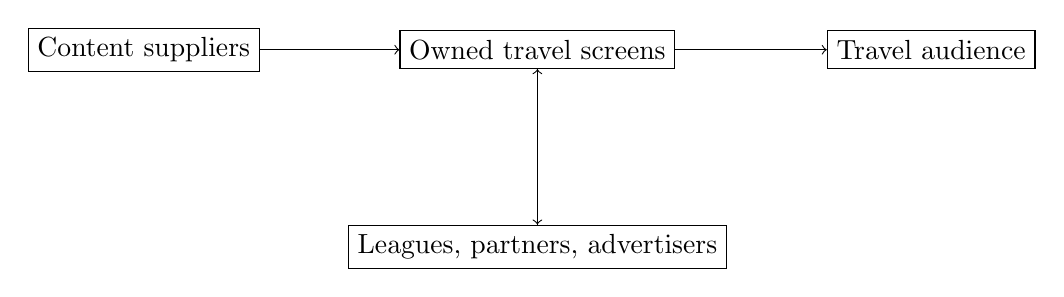
\begin{tikzpicture}
\node[draw, rectangle] (content) at (0,0) {Content suppliers};
\node[draw, rectangle] (network) at (5,0) {Owned travel screens};
\node[draw, rectangle] (aud) at (10,0) {Travel audience};
\node[draw, rectangle] (adv) at (5,-2.5) {Leagues, partners, advertisers};
\draw[->] (content) -- (network);
\draw[->] (network) -- (aud);
\draw[->] (adv) -- (network);
\draw[->] (network) -- (adv);
\end{tikzpicture}
\end{figure}

The important commercial move is that competitors and customers can overlap. The founder explicitly says that partners and customers include the very firms one might otherwise treat as competitors. Once again the lecture recovers the same deep idea we saw in dry cleaning, only at a different scale. If one controls the scarce interface through which others must pass, the boundary between rival and client becomes porous.

The founder's advice on selling and negotiating fits the same structure. Serve the person you are talking to. Never do something to someone; do something for someone. And when a prospective client leans toward no, interpret it not as a metaphysical impossibility but as a timing problem. The negotiation rule and the earlier Wall Street persistence rule are, at bottom, the same rule.

\section{Private Equity, Cash Flow, and the Final Finance Lens}

The final interview is analytically sharp in a different way. The guest is in private equity, not yet at a first million, and precisely because of that the lecture closes not with maximal wealth but with a more stripped-down financial grammar. What kind of businesses would one want if starting over? The answer is boring businesses with real cash flow, and financial-services businesses that can achieve scale.

\subsection{Question \& Answer}

\paragraph{Question.} If we were starting over, what exactly should we optimize for: glamour, a growth story, or cash that can actually be underwritten?

\paragraph{Answer.} The lecture's answer is unromantic. It prefers real assets, data centers, waste management, and similar businesses that generate actual dollars. The guest's specific contrast is between actual cash flow and EBITDA, the latter being described in the interview as ``kind of fake cash flow.'' The safe mathematical version of the point is this:
\begin{align}
CF_{\text{actual}} &\not\equiv E_{\text{EBITDA}}, \\
D_{\max} &= f(CF_{\text{actual}}), \qquad f' > 0.
\end{align}
That is to say, debt capacity is a function of actual cash generation, not of the most flattering accounting narrative.

The bank example sharpens the point further. Banks lend to make money, and they do so on the spread:
\begin{equation}
s_{\text{bank}} = r_{\text{loan}} - r_{\text{funding}}.
\end{equation}
This is standard finance, but in the lecture it is not presented as a textbook formula. It is given as a stripping-away of mystique. The speaker wants us to see the machine as a spread machine.

\begin{remark}
The dismissal of EBITDA in the interview is a heuristic, not an accounting theorem. The narrower and safer point is that lenders and buyers ultimately care about cash that can service obligations.
\end{remark}

The rest of the interview keeps translating broad entrepreneurial slogans into sharper financial language. Networking got him into private equity. Team quality is the real answer to competition. Finding deals and matching them with money is the scaling task. The most memorable line is that one should think about money the way one thinks about air. It is a metaphor, not an equation, but the meaning is exact enough: the desired state is one in which money is not worshipped one breath at a time because the system around it is already functioning.

This is also where the lecture's network motif reaches its cleanest statement. Your net worth is really your network, says the prior founder; the private-equity guest independently confirms the same principle in operational form. The shoes wear out, the phone number stays constant, the rooms matter. Relational capital is accumulated by showing up.

\section{Summary}

The lecture begins with a street question and ends with a finance vocabulary, but it never loses the order in which its ideas are earned. First we learn that access is scarce and persistence is part of the method. Then we are shown, in the dry-cleaning case, that scale often means separating the core process from the edge interface. Next we are told that a first million is not yet a stable system, because wealth preservation depends on the relation between recurring cash generation and drifting consumption. The surgeon adds a professional variant of the same story: quality, trust, referrals, and self-improvement over time. The Reach TV founder lifts the whole discussion to distribution, rights windows, and audience aggregation. The private-equity guest then closes the loop by asking us to underwrite actual cash, not vanity.

If one wants a single compact formula for the chapter, it is not a numerical identity but a structural one: durable wealth comes from repeatable systems. Those systems may take the form of a factory, a medical practice, a controlled distribution channel, or a portfolio of boring cash-flow businesses, but in every case the lecture pushes us away from spectacle and toward mechanism.